\documentclass[a4paper,10pt]{article}

% References
\usepackage[utf8]{inputenc}
\usepackage[style=bath,sorting=ynt,backend=biber]{biblatex}
\assignrefcontextentries[]{*}
\addbibresource{res/references.bib}

% Allow URLs in biblatex entries to break at lowercase characters
\setcounter{biburllcpenalty}{100}

% Asked for by biblatex
\usepackage{csquotes}

% Language and date format for UK english
\usepackage[british]{babel}
\usepackage[british]{isodate}
\cleanlookdateon

% Customise margin size
\usepackage[margin=1.4in]{geometry}

% Insertion of images
\usepackage{graphicx, float}
\graphicspath{{img/}}

% Automatic commands at the beginning of tabular rows (?)
\usepackage{array,etoolbox}

\newcounter{reqsec}
\newcounter{req}[reqsec]
\newcounter{subreq}[req]

\renewcommand{\thereq}{\thereqsec.\arabic{req}}
\renewcommand{\thesubreq}{\thereq.\arabic{subreq}}

\newcommand{\reqsec}[2]{\refstepcounter{reqsec}\thereqsec\label{#1}: #2}
\newcommand{\reqsection}[2]{%
  \toprule%
  \multicolumn{3}{l}{\textbf{%
    \reqsec{#1}{#2}%
  }} \\%
  \midrule%
}

\newcommand{\req}[1]{\refstepcounter{req}\thereq\label{#1}}
\newcommand{\requirement}[2]{%
  \req{#1}&%
  #2&%
}

\newcommand{\subreq}[1]{\refstepcounter{subreq}\thesubreq\label{#1}}
\newcommand{\subrequirement}[2]{%
  \subreq{#1}&
  #2&%
}

\newcommand{\priority}[1]{\emph{Priority:} #1\newline}
\newcommand{\phigh}{\priority{High}}
\newcommand{\pmed}{\priority{Medium}}
\newcommand{\plow}{\priority{Low}}

\newcommand{\deps}[1]{\emph{Dependencies:} #1\newline}
\newcommand{\dnone}{\deps{None}}
\newcommand{\source}[1]{\emph{Source:} #1\\}
\newcommand{\sspec}{\source{Coursework specification}}
\newcommand{\smin}[1]{\source{Meeting minutes \##1}}

\newenvironment{reqtable}
{\begin{longtable}{p{.07\textwidth} p{.43\textwidth} p{.40\textwidth}}}
{\bottomrule%
\end{longtable}}

\newcommand\reqheader{%
  \textbf{Index} & \textbf{Description} & \textbf{Priority, Dependencies, Source} \\%
  \midrule%
}

% Better horizontal lines for tables
\usepackage{booktabs}

% Tables that break over pages
\usepackage{longtable}

% Compact list environments
\usepackage{paralist}

% Add references to TOC
\usepackage[nottoc,numbib]{tocbibind}

% Strikethrough
\usepackage[normalem]{ulem}

% Allow insertion and numbering of appendices
\usepackage{appendix}

% Make links, section names, etc. clickable
\usepackage{hyperref}
% This must be the last package that is loaded!

\title{%
  CSED Group 11 Semester 2 Report \\
  \vspace{0.5em}
  \Large Computing as a Science and Engineering Discipline (CM10251)
}

\author{%
  Allington, Mathew \\
  \texttt{mma82@bath.ac.uk}
  \and
  Draper, Tom \\
  \texttt{td544@bath.ac.uk}
  \and
  Foot, Aethan \\
  \texttt{ajf75@bath.ac.uk}
  \and
  Ito-Low, Alexander \\
  \texttt{ail24@bath.ac.uk}
  \and
  Millischer, Christophe \\
  \texttt{cm2307@bath.ac.uk}
  \and
  Mortensen, Soren \\
  \texttt{snm48@bath.ac.uk}
  \and
  Sogbesan, Samuel \\
  \texttt{ss3222@bath.ac.uk}
  \and
  Songthammakul, Ravit \\
  \texttt{rs2347@bath.ac.uk}
}

\date{}

% Show down to subsubsection level in the main TOC
\setcounter{tocdepth}{3}

\begin{document}

\maketitle
\begin{abstract}
\end{abstract}

\vfill

\begin{center}
  \large Supervised by: \\
  \vspace{0.5em}
  Hyde, Jo \\
  \texttt{cssjkh@bath.ac.uk}
\end{center}

\newpage
\tableofcontents

\newpage
\section{Introduction}

\subsection{Overview of Domain}

% Personal informatics

Personal informatics is a term used to refer to devices and software that help people gather
information about themselves, so they can reflect upon it and gain motivation to make changes to
their lifestyle and habits to improve their overall wellbeing. Personal informatics is used for
effectively motivating people to gain self-knowledge, change behaviours. % Gen's source here

The area of personal informatics has started to expand in popularity in recent years mainly due to
the increased availability and usability of affordable hardware. Consumer products such as the
FitBit and Apple Watch allow users to collect data on a wide variety of metrics including heart
rate, blood pressure, motion and many others. Products such as the Neuroon, a wearable
electroencephalograph (EEG) eye mask, and Zeo Sleep Manager Pro, an EEG headband, allow the user to
collect information on brain waves for the purpose of sleep tracking.
% Validity of Consumer Activity Wristbands and Wearable EEG for Measuring Overall Sleep Parameters
% and Sleep Structure in Free-Living Conditions,

% Consumer Sleep Tracking Devices: A Critical Review in Digital Healthcare Empowering Europeans -
% write more here about other devices

Another factor that has contributed to the growth of personal informatics is the ubiquity of
smartphones, meaning that users have an ever-present device that allows them to collect and collate
data from their personal informatics hardware. Many personal informatics apps also add an element of
socially driven competition and gamification, driving users' motivation to continue to use them and
push their friends to also begin using this technology. In addition, there is a larger social force
pushing people to take steps to improve themselves. % Expand on this sentence

% Gamification!!

\subsection{Challenges}

Although personal informatics systems for wellbeing has been on the rise, it inherently presents
flaws that need to be taken into account. In a survey conducted by \textcite{Rapp:2014aa} where
participants were regular personal informatics users, it was revealed that the most significant
shortcomings of personal informatics systems supplied by commercial companies was a lack of
understanding for the end user's requirements and an absence of assistance and alerts for users who
didn't meet their goals. Apart from users who are familiar with personal informatics systems it is
also important to consider the challenges faced by the common user; a user who is new to using a
personal informatics device. It was discovered by \textcite{Rapp:2014aa} that the main challenge for
personal informatics systems was the lack of motivation faced by the end user to continue to use the
system. These challenges need to be taken into account because these hinder the end user from
improving themselves which is contradictory to the goal of personal informatics systems.

\subsubsection{Privacy and Security of Data}

% Data has to be stored somewhere, it's often being collected through third-party apps, no way to
% ensure it isn't transmitted or stored elsewhere

% Scraping of data with Cambridge Analytica, Strava military base heatmap

\subsubsection{Health Risks}

One crucial problem in the realm of health is sleep deprivation. Sleep deprivation is defined by the
\citeauthor{British-Medical-Association:2018aa} as ``a lack of sufficient sleep resulting from
disruption to the natural sleep cycle'' (\citeyear{British-Medical-Association:2018aa}). This is
important to highlight because as as opposed to fatigue, sleep deprivation isn't subjective. In
accordance to \textcite{Alhola:2007aa}, it was estimated that the main effect of sleep deprivation
was the reduction in cognitive performance. This includes: impaired attention; longer delays in
making decisions; poor quality of decisions and a reduction in long memory. This is especially
important to monitor for individuals who have high risk jobs. In 2010, 158 passengers' lives were
lost when an Air India Express plane overshot a runway by 600 metres. A leaked government report was
stated to have found that the accident unfolded due to the pilot's severe sleep deprivation
\parencite{British-Broadcasting-Corporation:2010aa}. Even in circumstances where the individual
isn't responsible for people's lives, a reduction in cognitive performance is still observed. Hence,
the validity of this problem is justified.

Sleep deprivation has the potential to be a dangerous to anyone and even fatal, if it is not
identified and managed. Over a third of adults get less than seven hours of sleep during a typical
24-hour period. Lack of sleep affects a person's abilities and health in many ways and can limit
their ability to perform in their line of work. This can be seriously, especially for professions
that the general public's lives rely on greatly such as doctors and nurses. Each year, 100,000
deaths occur in US hospitals due to medical errors and sleep deprivation in the medical staff has
been shown to contribute to this statistic \parencite{American-Sleep-Association:aa}. Driving whilst
feeling drowsy has been shown to be similar to driving whilst under the influence of alcohol and can
be attributed to a portion of car collisions each year
\parencite{National-Sleep-Foundation:aa}. There are few visible indications that an individual is
getting less sleep than recommended and it's difficult to know if you are deprived of sleep which
often makes it more damaging as it may be challenging to identify and then attempt to
curb. Similarly, there's no legal limit for sleep deprivation for situations such as driving a
vehicle. Sleep deprivation is difficult to measure without the aid of external equipment.

\subsubsection{Solution}

Our software system aims to reduce fatigue in individuals due to a lack of sleep. EEG have the
ability to detect sleeping problems based on brain wave patterns
\parencite{Mayfield-Certified-Health:2016aa}. Monitoring and recording the individual user's
brainwave data during their sleep allows the system to be tailored specifically for that
individual. Implementation of a points system would ensure the user regularly uses the headset. If
the system were to be used most nights, the headset would be able to measure and record a large
quantity of reliable data for the system to process making results recommendations the system
provides likely to be accurate and therefore helpful to the user. If the data were to be displayed
in a format easily, this would help the user to better understand their recorded sleep data and
allow them to make more appropriate decisions as to how to change their actions.

\section{Software requirements specification}\label{sec:srs}

\subsection{Problem domain and purpose of our system}\label{ssec:intro}
As mentioned earlier sleep deprivation is a prevalent problem that society faces.
When constructing the application we wanted it to be accessible to the general public as it was identified earlier that sleep deprivation has the potential to affect everyone.
It was identified that the main functionality of our system would be to aid users to track and compare their sleep through the Neuromind headset.

\subsection{Stakeholders involved and the elicitation process:}\label{ssec:stakeholders}
In order to elicit requirements, a questionnaire was constructed. Majority of the stakeholders involved were flight attendants from United Airlines.
In order to get a more diverse range of views to accomodate for diversity, an interview was conducted on a university student with a part time job.
Responses from participants validated our specific problem by justification both in the questionnaire and in the interviews.
We also constructed new requirements from group meetings through the agile process as group members working with specific requirements
identified that requirements could be refined to accomodate for a broader usage.

\subsection{How conflicts between requirements were managed:}\label{ssec:conflicts}
Throughout the course of the project, requirements were refined when group
meetings were conducted and observations by the group were made.
In particular, our team noticed that in order for the system to successfully calculate sleep cycle data,
it had to be extracted from the data calculated by the headset.

Another major requirement that was refined was the client interface.
This initially did not have any sub-requirements, but later sub-requirements had to be added in order for the stakeholder to be able to view processed data.
Without continuous communications between group members and stakeholder contact these optimisations would not have been possible.

Furthermore, towards the end of our project the client requirement remained, but another functional
requirement that we wanted to integrate into our software was the Graphical User Interface (GUI).
It had been expressed in the questionnaire that a graph to view sleep cycle data would be desirable for the end user.
Just having a Graphical user interface independent of the other functionalities would segment our system,
so as a group we devised to incorporate the GUI into our framework to ensure that it would be easier for
the user to interact with the system whilst maintaining a cohesive system.

\subsection{UseCase Diagram:}\label{ssec:UCD}
\begin{figure}[H]
  \centering
  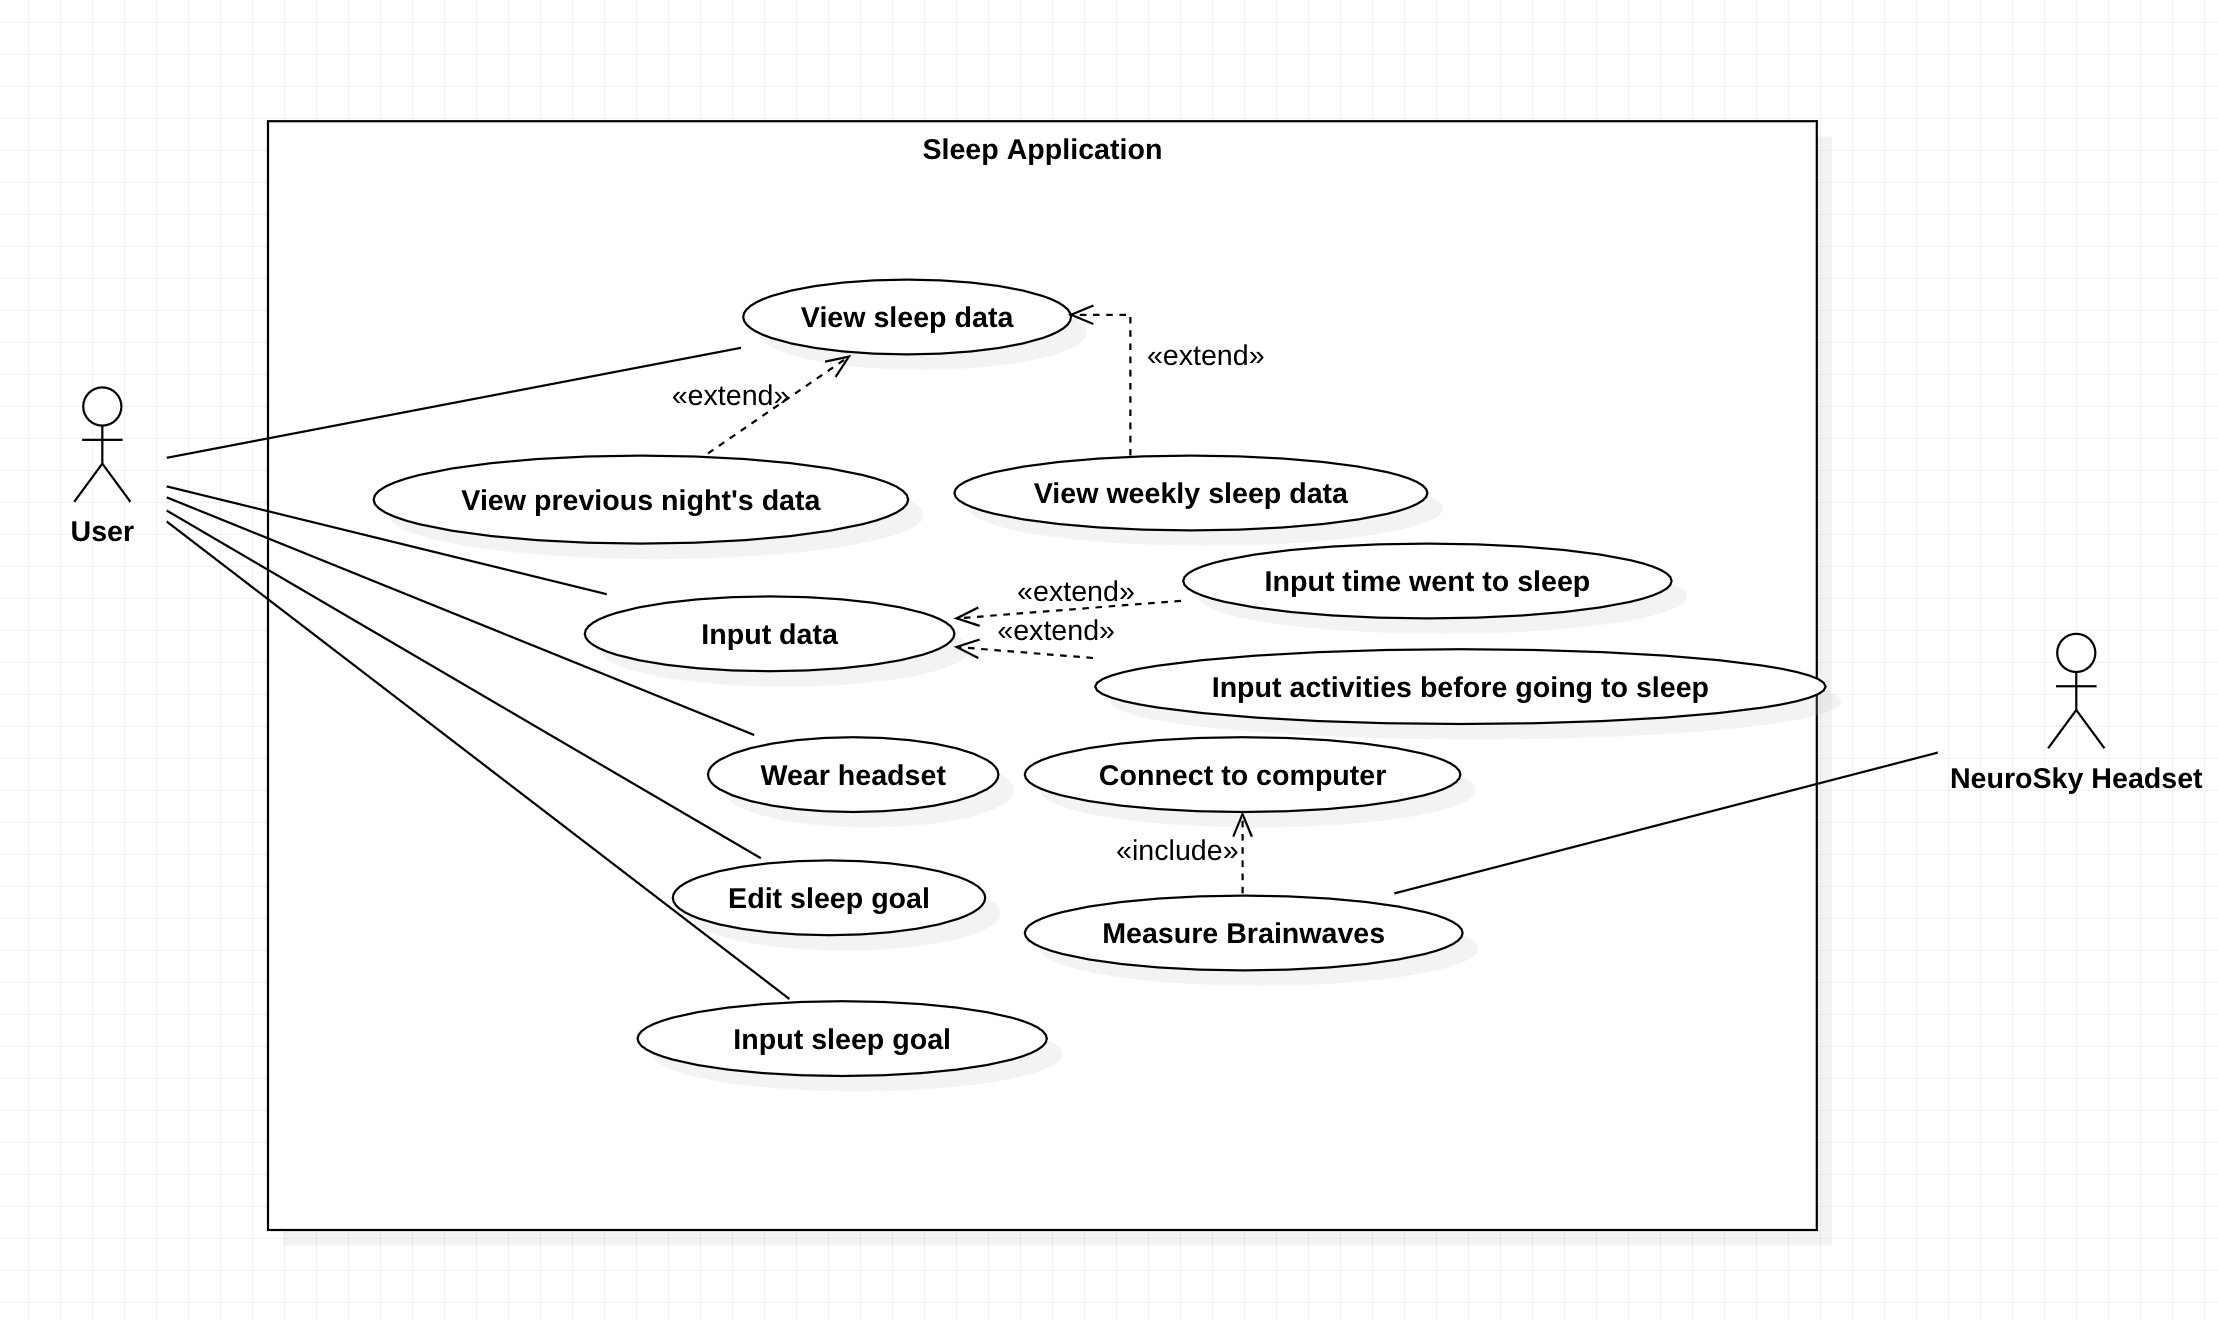
\includegraphics[width=1\textwidth]{UseCaseDiagram}
  \caption{Use Case Diagram}\label{img:use-case-diagram}
\end{figure}
Semantics:
The headset is the external hardware which the user has to wear in order to get a recording.
Once the user is wearing the headset, it can connect to the computer and then measure the user’s brainwaves.
The user is the general audience who will interact with our system.
The user can view sleep data they have inputted into the system using the headset.
They can view either their previous night’s data or last weeks data.
They can also set personal sleep goals which will allow them to then manage their goals that will be saved in the system.
They can also input the time they have previously went to sleep on nights they did not wear the headset.

\subsection{Scenarios:}\label{ssec:scenar}
\subsubsection{Scenario 1:}\label{ssec:scenar1}
Scenario 1:
Actor: User of the system
Goal: Measuring sleep data
Pre conditions:
  1. The user has neurosky headset
  2. The user has thinkgear socket connector installed on their laptop
  3. The user has our application installed.
\begin{figure}[H]
  \centering
  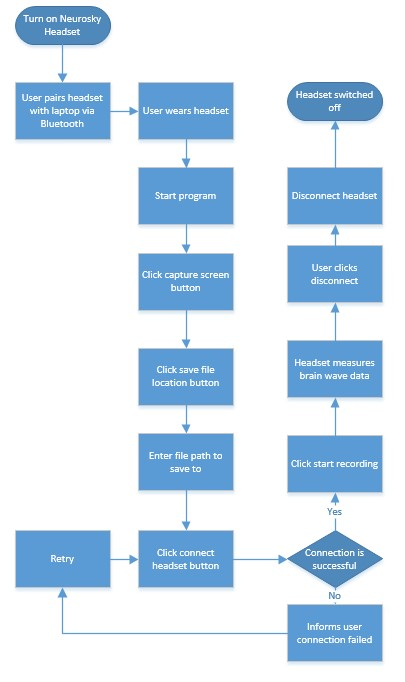
\includegraphics[width=0.5\textwidth]{UseCaseScenario1}
  \caption{Scenario 1}\label{img:usecasescenario1}
\end{figure}

\subsubsection{Scenario 2:}\label{ssec:scenar2}
Scenario 2:
Actor: The user of the system
Goal: View line graph of  brain activity throughout the time the headset was worn.
Preconditions:
The user has the application installed.
Scenario 1 has been completed at least once.
The user has already opened the application.
\begin{figure}[H]
  \centering
  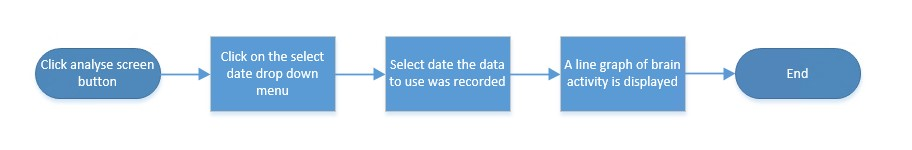
\includegraphics[width=1\textwidth]{UseCaseScenario2}
  \caption{Scenario 2}\label{img:usecasescenario2}
\end{figure}



\subsection{Non-Functional Requirements}\label{ssec:non-functional-requirements}

\renewcommand*{\arraystretch}{1.4}
\begin{reqtable}
  % Software Development Process

  \reqsection{reqs:soft-devel}{Software Development Process}
  \reqheader

  \requirement{req:agile-scrum}
  {The system must adhere to the Agile/Scrum methodology.}
  \phigh
  \dnone
  \sspec

  \requirement{req:3-sprints}
  {Software development should include at least 3 sprints.}
  \pmed
  \deps{\ref{req:agile-scrum}, \ref{req:1-3-weeks}}
  \sspec

  \requirement{req:1-3-weeks}
  {Each sprint should last between 1 and 3 weeks.}
  \pmed
  \deps{\ref{req:agile-scrum}, \ref{req:3-sprints}}
  \sspec

  \requirement{req:review-reqs}
  {Must review the functional requirements at every scrum meeting.}
  \phigh
  \deps{\ref{req:1-3-weeks}}
  \sspec

  \requirement{req:risk-management}
  {Must incorporate risk management into the software process.}
  \phigh
  \deps{\ref{req:agile-scrum}}
  \sspec

  % Expanding Initial Requirements

  \reqsection{reqs:expanding-initial}{Expanding Initial Requirements}
  \reqheader

  \requirement{req:expand-non-func}
  {The system must expand upon the initial non-functional requirements.}
  \phigh
  \dnone
  \sspec

  \requirement{req:expand-func}
  {The system must expand upon the initial functional requirements and add additional functionality
    to the system.}
  \phigh
  \dnone
  \sspec

  \requirement{req:additional-reqs}
  {Additional requirements should be established by conducting interviews on potential users,
    reading articles on personal informatics and examining existing personal informatics systems.}
  \phigh
  \deps{\ref{req:expand-non-func}, \ref{req:expand-func}}
  \sspec

  % Background Research

  \reqsection{reqs:background-research}{Background Research}
  \reqheader

  \requirement{req:4-articles}
  {Must read and cite 4 articles in the field of personal informatics.}
  \phigh
  \dnone
  \sspec

  \requirement{req:8-articles}
  {Should read and cite at least eight articles.}
  \pmed
  \dnone
  \sspec

  \requirement{req:core-peer-reviewed}
  {Citations of core article must be peer-reviewed articles.}
  \phigh
  \deps{\ref{req:4-articles}}
  \sspec

  \requirement{req:additional-web}
  {Additional citations may be made to web articles of unknown quality.}
  \plow
  \dnone
  \sspec

  \requirement{req:classify-rem-cycles}
  {Must classify measurements of stages of sleep (REM cycles).}
  \phigh
  \dnone
  \source{\textcite{Tuck:2018aa}, \textcite{Feinberg:1988aa}, \textcite[p.291]{Carlson:2012aa}}

  % Ethical Issues

  \reqsection{reqs:ethical-issues}{Ethical Issues}
  \reqheader

  \requirement{req:ethical-issues}
  {Must account for ethical issues in the specification, design, development and testing of the
    system.}
  \phigh
  \dnone
  \sspec

  % Testing

  \reqsection{reqs:testing}{Testing}
  \reqheader

  \requirement{req:test-driven-approach}
  {Must adopt a test-driven development approach with production of test plans.}
  \phigh
  \dnone
  \sspec

  \requirement{req:evidence-testing}
  {Must provide evidence of testing.}
  \phigh
  \dnone
  \sspec

  \requirement{req:state-hypothesis}
  {Must state hypothesis which clearly link claims to observable behaviours of your system in
    operation.}
  \phigh
  \dnone
  \sspec

  \requirement{req:valid-analysis}
  {Must conduct a valid analysis of empirical data generated from an experiment (should include
    Student's t-test).}
  \phigh
  \dnone
  \sspec
\end{reqtable}

\subsection{Functional Requirements}\label{ssec:functional-requirements}

\begin{reqtable}
  % Viewing and Collecting Sleep Data

  \reqsection{reqs:viewing-collecting-data}{Viewing and Collecting Sleep Data}
  \reqheader

  \requirement{req:interface-headset}
  {The system must be able to interface with the Neurosky headset.}
  \phigh
  \deps{\ref{sreq:connect-headset}, \ref{sreq:disconnect-headset}, \ref{sreq:read-data-headset}}
  \smin{12}

  \subrequirement{sreq:connect-headset}
  {The system must be able to connect to the Neurosky headset.}
  \phigh
  \dnone
  \smin{9}

  \subrequirement{sreq:disconnect-headset}
  {The system must be able to disconnect from the Neurosky headset.}
  \phigh
  \deps{\ref{sreq:connect-headset}}
  \smin{9}

  \subrequirement{sreq:read-data-headset}
  {The system must be able to read in raw brainwave data from the Neurosky headset.}
  \phigh
  \deps{\ref{sreq:connect-headset}}
  \smin{7}

  \requirement{req:store-data}
  {The system must store raw brainwave data.}
  \phigh
  \deps{\ref{sreq:facilitate-saving}, \ref{sreq:facilitate-conversion}}
  \source{Coursework specification, meeting minutes \#7}

  \subrequirement{sreq:facilitate-saving}
  {The system must facilitate the saving of converted brainwave data to a binary file (.ec).}
  \phigh
  \deps{\ref{sreq:read-data-headset}}
  \smin{12}

  \subrequirement{sreq:facilitate-conversion}
  {The system must facilitate the conversion of brainwave data from binary (.ec) to CSV format.}
  \phigh
  \deps{\ref{sreq:facilitate-saving}}
  \smin{12}

  \requirement{req:extract-data}
  {The system should be able to extract information about sleep cycles from recorded raw data.}
  \phigh
  \deps{\ref{sreq:extract-attention-meditation}, \ref{sreq:calculate-moving-average}}
  \smin{13}

  \subrequirement{sreq:extract-attention-meditation}
  {The system should extract the attention and meditation data points from the raw brainwave data.}
  \phigh
  \deps{\ref{req:store-data}}
  \smin{16}

  \subrequirement{sreq:calculate-moving-average}
  {The system should calculate a moving average of the attention and meditation values for the whole
    data set.}
  \phigh
  \deps{\ref{sreq:extract-attention-meditation}}
  \smin{16}

  \subrequirement{sreq:extract-sleep-percentage}
  {The system must extract the percentage of time during a recording when the user was asleep vs.\
    awake.}
  \phigh
  \deps{\ref{sreq:calculate-moving-average}}
  \smin{16}

  \requirement{req:present-data}
  {The system should be able to present sleep cycle data to the user.}
  \phigh
  \deps{\ref{sreq:present-data-table},\ref{sreq:present-hypnogram}}
  \source{Coursework specification, meeting minutes \#7, sleep app questionnaire}

  \subrequirement{sreq:present-data-table}
  {The system should be able to present sleep cycle data in the form of a data table.}
  \phigh
  \deps{\ref{req:extract-data}}
  \smin{17}

  \subrequirement{sreq:present-hypnogram}
  {The system should be able to present sleep cycle data in the form of a line graph.}
  \phigh
  \deps{\ref{req:extract-data}}
  \source{Sleep app questionnaire}

  \requirement{req:manual-entry}
  {The system should permit the manual entering of relevant user data from the last 24 hours.}
  \pmed
  \deps{\ref{req:manual-entry-bed-woke}}
  \source{Coursework specification, sleep app questionnaire,
    \textcite{British-Medical-Association:2018aa}}

  \subrequirement{req:manual-entry-bed-woke}
  {The system must permit the manual entry of information that corresponds to the times when the
    user went to bed and woke up.}
  \pmed
  \dnone
  \source{\textcite{British-Medical-Association:2018aa}, sleep app questionnaire}

  \requirement{req:apply-sorting-algorithm}
  {The system should apply a ``known'' sorting algorithm which allows users to sort tracking data}
  \pmed
  \deps{\ref{req:store-data}}
  \sspec

  \requirement{req:implement-cli}
  {The system should implement a command-line interface allowing the user to perform all functions
    of the system.}
  \phigh
  \deps{\ref{sreq:allow-user-record-data}, \ref{sreq:specify-time-record},
    \ref{sreq:allow-user-change-format}, \ref{sreq:allow-user-extract-calculate},
    \ref{sreq:cli-sort-display}}
  \smin{13}

  \subrequirement{sreq:allow-user-record-data}
  {The command-line interface should allow the user to record data from the headset and choose where
    to store it.}
  \phigh
  \deps{\ref{sreq:read-data-headset}, \ref{sreq:facilitate-saving}}
  \smin{13}

  \subrequirement{sreq:specify-time-record}
  {The command-line interface should allow the user to specify an amount of time to record for, in
    minutes or in seconds.}
  \phigh
  \deps{\ref{sreq:allow-user-record-data}}
  \smin{13}

  \subrequirement{sreq:allow-user-change-format}
  {The command-line interface should allow the user to convert a binary (.ec) file to CSV format,
    and choose where to save the converted file.}
  \phigh
  \deps{\ref{sreq:facilitate-conversion}}
  \smin{13}

  \subrequirement{sreq:allow-user-extract-calculate}
  {The command-line interface should allow the user to extract and calculate a moving average of the
    attention and meditation data.}
  \phigh
  \deps{\ref{sreq:calculate-moving-average}}
  \smin{16}

  \subrequirement{sreq:cli-process-sleep-data}
  {The command line interface must allow the user to process sleep cycle data from a raw recorded
    data file.}
  \phigh
  \deps{\ref{sreq:extract-sleep-percentage}}
  \smin{16}

  \subrequirement{sreq:cli-sort-display}
  {The command line interface must display processed sleep cycle data in the form of a table.}
  \phigh
  \deps{\ref{req:apply-sorting-algorithm}}
  \smin{13}

  % Identifying Trends in Data

  \reqsection{reqs:identifying-trends-data}{Identifying Trends in Data}
  \reqheader

  \requirement{req:compare-sleep-data}
  {The system must allow the user to compare sleep data over a week.}
  \phigh
  \deps{\ref{req:store-data}, \ref{req:manual-entry}}
  \source{\textcite{British-Medical-Association:2018aa}, sleep app questionnaire}

  \requirement{req:Automation-of-data}
  {The system should permit the creation of automated data based on the user's sleep cycle}
  \pmed
  \deps{\ref{req:store-data}}
  \smin{12}

  % Goals and Achievements

  \reqsection{reqs:goals-achievements}{Goals and Achievements}
  \reqheader

  \requirement{req:allow-manage-goals}
  {Allow users to manage targets (goals) for time going to bed.}
  \pmed
  \deps{\ref{req:store-data}, \ref{req:manual-entry}}
  \source{Coursework specification, sleep app questionnaire}

  \requirement{req:permit-set-goal}
  {Should permit user to set a daily or weekly goal for time going to bed.}
  \pmed
  \dnone
  \source{Coursework specification, meeting minutes \#7}

  \requirement{req:update-change-goal}
  {Should permit user to update or change goal.}
  \pmed
  \dnone
  \sspec

  \requirement{req:motivate-user}
  {Should motivate user to achieve their goals via a point system.}
  \pmed
  \deps{\ref{req:allow-manage-goals}, \ref{req:permit-set-goal}}
  \source{Coursework specification, sleep app questionnaire}

  % Manage Data Periodically

  \reqsection{reqs:manage-data-periodically}{Manage Data Periodically}
  \reqheader

  \requirement{req:delete-data}
  {Users should be given the option to delete their sleep cycle data}
  \plow
  \deps{\ref{req:store-data}, \ref{req:extract-data}}
  \source{Meeting minutes \#13, sleep app questionnaire}
\end{reqtable}

% \include{tex/design}
% \include{tex/conclusions}

\section{References}
\newrefcontext[sorting=nyt]
\printbibliography[heading=none]

% \include{tex/group-contribution-form}

% \begin{appendices}
%   \include{tex/draft-hlas}
%   \include{tex/state-machine}
%   \include{tex/meeting-minutes}
% \end{appendices}

\end{document}
